\section{CMMI}
Il \textbf{Capability Maturity Model Integration} è un approccio al miglioramento dei processi organizzativi al fine di migliorare le prestazioni. Fondamento del CMMI è la valutazione dei processi e la classificazione in livelli di maturità degli stessi al fine di giudicare un sistema, o un intera azienda. Possiamo definire ogni singolo elemento del CMMI:
\begin{itemize}
	\item \textbf{Capability}: misura la capacità del sistema di raggiungere gli scopi a esso assegnato, può essere  in quattro livelli:
	\begin{itemize}
		\item Incompleto: approccio incompleto per raggiungere l'obiettivo;
		\item Initial: approccio iniziale per soddisfare gli obiettivi, non è una serie soddisfacente di pratiche necessarie;
		\item Managed: completa e semplice serie di pratiche che soddisfano l'intento generale;
		\item Definita: si basa su pratiche standardizzate che organizzano e personalizzano il sistema di lavoro e di gestione.
	\end{itemize}	 
	\item \textbf{Maturity}: misura quanto l'azienda è governata dal suo sistema di processi; la maturità può essere classificata in cinque livelli:
	\begin{itemize}
		\item Initial: il lavoro non è organizzato ed è imprevedibile e reattivo, porta spesso a ritardi e sforamento del budget;
		\item Managed: il lavoro è gestito, controllato e misurato a livello di progetto, si può considerare ancora un livello basato sulla ricerca reattiva di una eventuale soluzione;
		\item Defined: il lavoro è proattivo piuttosto che reattivo, gli standard a livello organizzativo gestiscono programmi e portfogli;
		\item Quantitatively Managed: il lavoro è misurato e controllato, l'organizzazione è guidata con obiettivi di miglioramento delle prestazioni prevedibili e allineati per soddisfare gli stakeholder;
		\item Optimizing: il lavoro è stabile e flessibile, l'organizzazione è focalizzata al miglioramento continuo ed è studiare per ruotare e cambiare a seconda del contesto ; la stabilità offre una piattaforma che permette innovazione e agilità.
	\end{itemize}
	\item \textbf{Model}: criteri per la valutazione del grado di qualità dei processi di validazione;
	\item \textbf{Integration}: architettura di integrazione delle diverse discipline e tipologie di attività delle aziende:
	\begin{itemize}
		\item CMMI-DEV: sviluppo prodotti;
		\item CMMI-SVC: gestione dei servizi;
		\item CMMI-ACQ: acquisto prodotti e servizi esterni.
	\end{itemize}	 
\end{itemize}
Il CMMI si può definire un framework che ottiene benefici maggiori in aziende di medie-grandi dimensione, circa il 50\% delle aziende che hanno tra i 1000 e i 2000 dipendenti si collocano al livello massimo di maturità, mentre il 70\% delle aziende con in media 25 dipendeti si collocano al livello 2.

\begin{figure}[H]
\centering
	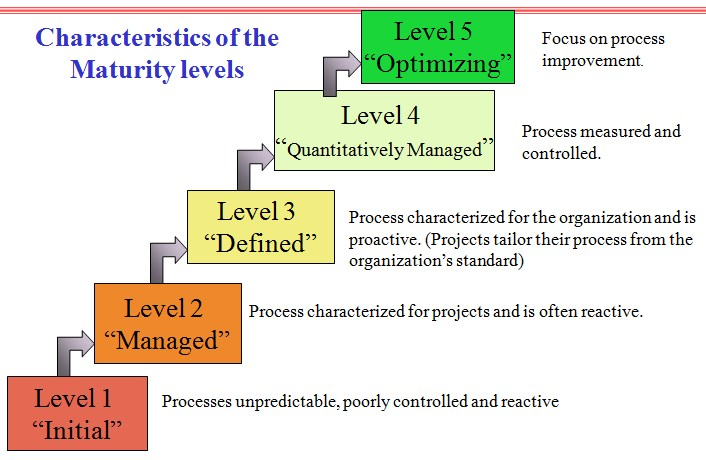
\includegraphics[width=0.7\linewidth]{./images/Characteristics_of_the_Maturity_levels.jpg} 
	\caption{Capability Maturity Model Integration - CMMI}
	\label{cmmi}
\end{figure}


